\documentclass[11pt]{article}

\usepackage[margin=1.05in]{geometry}
\usepackage[T1]{fontenc}
\usepackage{mathpazo}
\usepackage[scaled=0.92]{helvet}
\usepackage{courier}
\usepackage{amsmath,amssymb,mathtools,bm}
\usepackage{booktabs,array,multirow}
\usepackage{enumitem}
\usepackage{xcolor}
\usepackage{graphicx}
\usepackage{tikz}
\usepackage{tcolorbox}
\usepackage{titlesec}
\usepackage{caption}
\usepackage{microtype}
\usepackage{needspace}
\usepackage[hidelinks]{hyperref}

\usetikzlibrary{positioning,arrows.meta,calc}
\tcbuselibrary{skins,breakable}

% ---------------------------------------------------------------- palette
\definecolor{navy}{RGB}{25,55,92}
\definecolor{muted}{RGB}{90,96,105}
\definecolor{rule}{RGB}{200,201,196}
\definecolor{okgreen}{RGB}{0,110,60}
\definecolor{specblue}{RGB}{42,120,214}
\definecolor{newmag}{RGB}{160,45,120}
\definecolor{openamber}{RGB}{170,110,0}
\definecolor{limred}{RGB}{175,45,45}
\definecolor{tint}{RGB}{248,248,246}
\definecolor{lg}{RGB}{175,177,172}

% ---------------------------------------------------------------- headings
\titleformat{\section}{\normalfont\sffamily\large\bfseries\color{navy}}{\thesection}{0.7em}{}
\titleformat{\subsection}{\normalfont\sffamily\normalsize\bfseries\color{navy}}{\thesubsection}{0.6em}{}
\titleformat{\part}[display]
  {\normalfont\sffamily\Large\bfseries\color{navy}\filcenter}
  {\MakeUppercase{\partname~\thepart}}{0.4em}{}
\titlespacing*{\section}{0pt}{1.5em}{0.6em}
\titlespacing*{\subsection}{0pt}{1.2em}{0.45em}

% ---------------------------------------------------------------- macros
\newcommand{\R}{\mathbb{R}}
\newcommand{\Prob}{\mathbb{P}}
\newcommand{\Ind}{\mathbf{1}}
\newcommand{\dhat}{\hat{d}}
\newcommand{\pihat}{\hat{\pi}}
\newcommand{\nhat}{\hat{n}}
\newcommand{\chat}{\hat{c}}
\newcommand{\that}{\hat{t}}
\newcommand{\Dhat}{\hat{\Delta}}

\newcommand{\provtag}[2]{{\footnotesize\sffamily\textcolor{#1}{[#2]}}}
\newcommand{\VALID}{\provtag{okgreen}{VALIDATED}}
\newcommand{\SPEC}{\provtag{specblue}{SPECIFIED}}
\newcommand{\NEWT}{\provtag{newmag}{NEW}}
\newcommand{\OPENT}{\provtag{openamber}{OPEN}}
\newcommand{\LIMIT}{\provtag{limred}{LIMIT}}

\newcommand{\why}[1]{\par\smallskip\noindent\textcolor{muted}{\small\itshape #1}\par\smallskip}

\newtcolorbox{claimbox}[1][]{
  enhanced, breakable, colback=tint, colframe=navy, boxrule=0pt,
  leftrule=2.5pt, arc=0pt, outer arc=0pt,
  left=12pt, right=12pt, top=9pt, bottom=9pt, #1}

\newtcolorbox{resultbox}[1][]{
  enhanced, breakable, colback=okgreen!4, colframe=okgreen!55, boxrule=0pt,
  leftrule=2.5pt, arc=0pt, outer arc=0pt,
  left=12pt, right=12pt, top=9pt, bottom=9pt, #1}

\newtcolorbox{limitbox}[1][]{
  enhanced, breakable, colback=limred!4, colframe=limred!55, boxrule=0pt,
  leftrule=2.5pt, arc=0pt, outer arc=0pt,
  left=12pt, right=12pt, top=9pt, bottom=9pt, #1}

\newtcolorbox{codebox}[1][]{
  enhanced, breakable, colback=tint, colframe=rule, boxrule=0.5pt,
  arc=2pt, left=10pt, right=8pt, top=7pt, bottom=7pt,
  fontupper=\footnotesize\ttfamily, #1}

\newtcolorbox{notebox}[1][]{
  enhanced, breakable, colback=white, colframe=rule, boxrule=0.5pt,
  arc=2pt, left=10pt, right=10pt, top=7pt, bottom=7pt,
  fontupper=\small, #1}

\captionsetup{font=small,labelfont={sf,bf,color=navy}}
\setlist[itemize]{leftmargin=1.3em,itemsep=2pt,topsep=4pt}
\setlist[enumerate]{leftmargin=1.6em,itemsep=2pt,topsep=4pt}
\renewcommand{\arraystretch}{1.15}

\hypersetup{
  pdftitle={Recovering a Hidden Routing Boundary from Query-Only Access},
  pdfauthor={Robert Romani},
  pdfsubject={Method note v5},
}

\title{\textcolor{navy}{\sffamily Recovering a Hidden Routing Boundary\\[2pt]
from Query-Only Access}\\[6pt]
\large\normalfont Method note, v5}
\author{Robert Romani}
\date{August 13, 2026}

\begin{document}
\maketitle

\begin{abstract}
\noindent Given query access to a deployed model and a set of real inputs, we estimate the
\emph{geometry} of a hidden routing rule. Around each anchor we send a probe cloud shaped by
the local data geometry, remove within-branch trend with a trimmed local-linear fit, and test
the residual distribution for a two-component structure whose components are linearly separable
in input space. From the fitted mixture, its \emph{weight} gives the distance to the boundary and
its \emph{separating direction} gives the boundary's normal; both are checked for consistency
across a scale ladder. Pooling these local estimates across anchors---weighted by evidence
rather than thresholded---yields a single hyperplane with a confidence interval and a
permutation-calibrated $p$-value, and where that hyperplane is axis-dominated, the coordinate
and threshold the system routes on. We characterise where this is identifiable and where it
provably is not.

\medskip
\noindent\textcolor{muted}{\small This note supersedes \texttt{pipeline\_v4} and the Stage~0/1
description in \texttt{probe\_policy\_spec}. The change is structural rather than additive: v4
described a detector with recovery appended. This document is organised around the object being
estimated---the boundary---and treats every earlier stage as part of the argument that the
estimate is trustworthy.}
\end{abstract}

\noindent\textbf{\sffamily\small\textcolor{navy}{Provenance tags used throughout.}}
\smallskip

{\small
\begin{tabular}{@{}ll@{}}
\VALID & measured against ground truth\\
\SPEC & designed in detail, not implemented\\
\NEWT & introduced in this note\\
\OPENT & acknowledged gap\\
\LIMIT & structural impossibility, not expected to yield to engineering\\
\end{tabular}}

\vspace{0.5em}

\part{What the method claims}

\section{The target sentence}
\label{sec:target}

A deployed model may contain a hidden switch: one rule on some inputs, a different rule on
others, with nothing in the interface saying so. We have query access only---no weights, no
gradients, no routing metadata, no labels.

The claim we want to end up making is not \emph{``something looks suspicious here.''} It is:

\begin{claimbox}
\noindent The system routes on coordinate $i$ at threshold $\that = 4.98 \pm 0.07$, recovered
from $N$ anchors under query-only access, $p < 0.05$ against a permutation null.
\end{claimbox}

\noindent That is an \emph{inverse problem}, not a test. The question is not ``does hidden
routing happen''---several published methods answer that. The question is \emph{``given only the
system's outputs, what can I infer about the mechanism that produced them.''} Everything in this
note exists to make that sentence defensible.

\section{The idea, in words}
\label{sec:idea}

Pick a real input $x$---call it an \textbf{anchor}. Send a small cloud of nearby queries and look
at the answers.

If the anchor sits well inside one routing region, every probe gets the same rule and the answers
vary smoothly. If the anchor sits near a boundary, some probes land on the far side and get a
\emph{different} rule. Those answers are shifted by a constant---the penalty $\Delta$---so the
response distribution splits into two clumps rather than one spread.

Three quantities fall out of that split, and each says something different.

\begin{itemize}
\item \textbf{How many probes crossed} tells you \textbf{how far away the boundary is.} If 5\% of
probes crossed, the boundary is far relative to the probe radius; if 40\% crossed, it is close.
The Gaussian geometry converts one into the other exactly.
\item \textbf{Where the crossers sit} tells you \textbf{which way the boundary faces.} The mixture
model labels each probe as probably-branch-1 or probably-branch-2. Plot those labels back in input
space and fit the separating plane; its perpendicular is the boundary's direction.
\item \textbf{Agreement across anchors} tells you \textbf{whether they are all seeing the same
boundary}, and pooling many noisy local planes gives one global plane with error bars.
\end{itemize}

\begin{figure}[h]
\centering
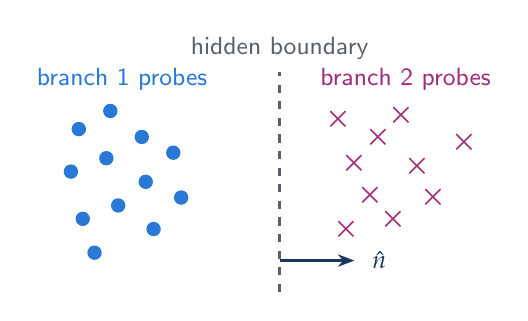
\begin{tikzpicture}[scale=1.0]
% boundary
\draw[dashed,thick,muted] (0,-1.35) -- (0,1.45);
\node[muted,font=\small\sffamily] at (0,1.75) {hidden boundary};
% branch 1 dots
\foreach \x/\y in {-2.55/0.72, -2.15/0.95, -1.75/0.62, -2.65/0.18, -2.2/0.35,
                   -1.7/0.05, -2.5/-0.42, -2.05/-0.25, -1.6/-0.55, -2.35/-0.85,
                   -1.35/0.42, -1.25/-0.15}
  \fill[specblue] (\x,\y) circle (2.6pt);
% branch 2 crosses
\foreach \x/\y in {0.75/0.85, 1.25/0.62, 0.95/0.28, 1.55/0.9, 1.15/-0.12,
                   1.75/0.25, 0.85/-0.55, 1.45/-0.42, 1.95/-0.15, 2.35/0.55}
  \node[newmag,inner sep=0pt,font=\normalsize\bfseries] at (\x,\y) {$\bm{\times}$};
% normal arrow
\draw[-{Stealth[length=6pt]},thick,navy] (0,-0.95) -- (0.95,-0.95);
\node[navy,font=\small\sffamily,anchor=west] at (1.05,-0.95) {$\nhat$};
% labels
\node[specblue,font=\small\sffamily] at (-2.0,1.35) {branch 1 probes};
\node[newmag,font=\small\sffamily] at (1.6,1.35) {branch 2 probes};
\end{tikzpicture}
\caption{One anchor. The responses say, probabilistically, which side each probe fell on. The
plane separating those two groups \emph{in input space} has the boundary's orientation; its
perpendicular is $\nhat$.}
\end{figure}

One anchor gives a noisy local estimate. Repeat around many anchors and pool.

\begin{figure}[h]
\centering
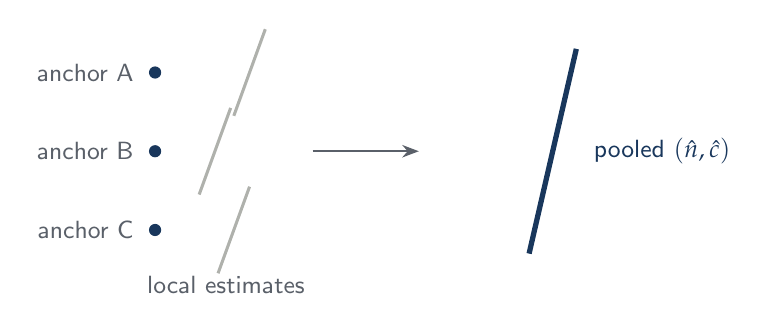
\begin{tikzpicture}[scale=1.0]
% local estimates
\foreach \y/\off in {1.15/0.30, 0.15/-0.14, -0.85/0.10}{
  \fill[navy] (-3.2,\y) circle (2.2pt);
  \draw[lg,line width=1.1pt] (-2.5+\off,\y-0.55) -- (-2.1+\off,\y+0.55);
}
\node[font=\small\sffamily,anchor=east,muted] at (-3.35,1.15) {anchor A};
\node[font=\small\sffamily,anchor=east,muted] at (-3.35,0.15) {anchor B};
\node[font=\small\sffamily,anchor=east,muted] at (-3.35,-0.85) {anchor C};
% arrow
\draw[-{Stealth[length=6pt]},thick,muted] (-1.2,0.15) -- (0.15,0.15);
% pooled
\draw[navy,line width=1.9pt] (1.55,-1.15) -- (2.15,1.45);
\node[navy,font=\small\sffamily,anchor=west] at (2.25,0.15) {pooled $(\nhat,\chat)$};
\node[muted,font=\small\sffamily] at (-2.3,-1.55) {local estimates};
\end{tikzpicture}
\caption{Many anchors. Local planes that are individually noisy pool into one global plane. If
the pooled normal is dominated by a single coordinate, the rule is axis-aligned and can be stated
as a feature and a threshold.}
\end{figure}

\section{A worked example, end to end}
\label{sec:example}

Suppose the true hidden rule is $g(x) = \Ind[x_3 \ge 5]$. You do not know this.

You pick an anchor with $x_3 = 4.7$ and probe with per-coordinate scale $\sigma = 0.5$.

\begin{description}[leftmargin=0pt,style=unboxed,itemsep=5pt]
\item[\textnormal{\textbf{1. The mixture.}}] The two-component fit returns $\pihat = 0.27$: about
27\% of probes landed on the other branch.

\item[\textnormal{\textbf{2. Distance.}}] The signed displacement along any unit direction is
$N(0,\sigma^2)$, so the crossing fraction is $\Phi(-d/\sigma)$. Invert it:
\[
  \dhat \;=\; -\sigma\,\Phi^{-1}(\pihat) \;=\; -0.5 \cdot \Phi^{-1}(0.27)
        \;=\; -0.5 \cdot (-0.613) \;=\; 0.31 .
\]
The true distance is $5 - 4.7 = 0.30$. \emph{You have just measured how far away an unobservable
boundary is, from nothing but the proportion of a mixture.}

\item[\textnormal{\textbf{3. Direction.}}] The probes assigned to the second component are mostly
those where $x_3$ increased. The classifier separating the components returns
$\nhat \approx (0,0,1,0,\dots)$. Note the distance was \emph{unsigned}---the crossing law gives
magnitude only, and the direction comes from $\nhat$. You need both.

\item[\textnormal{\textbf{4. Offset.}}] Anchor at $x_3 = 4.70$, $0.31$ away in the $+x_3$
direction: $\chat = 4.70 + 0.31 = 5.01$.

\item[\textnormal{\textbf{5. Pool.}}] Do this at 100 anchors and combine. You might land at
$\nhat = (0.01,-0.02,0.999,0.01,\dots)$ and $\chat = 4.98 \pm 0.07$---and the claim in
\S\ref{sec:target} is now supported by evidence.
\end{description}

\section{Why the earlier stages exist}
\label{sec:why}

Steps 1--5 above are the whole scientific content, and every one of them can be wrong for a
reason that has nothing to do with routing. The rest of the pipeline is the list of those
reasons and what stops each.

\begin{table}[h]
\small
\begin{tabular}{@{}p{0.52\textwidth}p{0.42\textwidth}@{}}
\toprule
\textbf{\sffamily What could go wrong} & \textbf{\sffamily What stops it}\\
\midrule
The probe ball never reaches the boundary, so there is nothing to see
  & \textbf{Stage 0} --- bound the radius by the geometry, and report when no valid radius exists\\
The probes land where no real input occurs, so the ``gate'' is real in input space but never
fires in deployment
  & \textbf{Stage 1} --- density filter\\
The probe cloud inherits the \emph{data's} clumpiness and reads as two branches under a
perfectly smooth model
  & \textbf{Stage 1} --- a smooth cloud in the tangent frame is unimodal by construction\\
A smooth trend across the ball masks the jump---or worse, the fitted plane eats it
  & \textbf{Stage 2} --- trimmed residualisation\\
Ordinary curvature produces a lopsided residual distribution that a mixture fits better than one
Gaussian
  & \textbf{Stage 3} --- the separability guard, plus the checks in Stage 5\\
The mixture is real but it is not a \emph{boundary}---components interleaved in space
  & \textbf{Stage 3} --- separability again\\
The local estimates are individually too noisy to trust
  & \textbf{Stage 6} --- pool, weighting by evidence rather than thresholding\\
\bottomrule
\end{tabular}
\end{table}

\noindent So the stages are not scaffolding around a detector. They are the reasons a reader
should believe $(\nhat,\chat)$.

\part{The machinery}

\section{Setup and standing assumptions}
\label{sec:setup}

\[
  y \;=\; f_{g(x)}(x) + \varepsilon, \qquad \varepsilon \sim N(0,\tau^2),
  \qquad g:\mathcal{X}\to\{1,2\} \ \text{hidden}, \qquad g(x)=\Ind[w^\top x > b].
\]

Crossing swaps branch and shifts the output by an additive $\Delta$. Routing is \textbf{top-1 and
hard}---the entering branch arrives at full weight, so the output \emph{steps}. Top-2 softmax
routing instead produces a \emph{kink}: the output stays continuous and only the derivative jumps.
That is out of scope, and \S\ref{sec:stage5} shows the distinction is detectable rather than
assumed.

An anchor set $A$ is drawn from the deployment distribution and \textbf{fixed before any query to
$f$}. This is not a convenience: it is what makes the adaptive scale selection in Stage~0 free of
any selection penalty. If anchors were chosen using earlier responses, the argument collapses.

\section{Stage 0 --- where is it legitimate to probe?}
\label{sec:stage0}

\begin{notebox}
\textbf{\sffamily Status.} Specified, not implemented, and deliberately deferred below the
critical path---see \S\ref{sec:path}. The recovery results are established first with the frame
and radius \emph{supplied}; this stage is what later lets the method choose them for itself.
\end{notebox}

\smallskip
\noindent Reads anchor covariates only; never touches $f$. Costs zero queries.

The probe radius must satisfy two things that pull against each other: big enough to reach the
boundary, small enough that the honest surface is roughly flat over the ball so the plane fitted
in Stage~2 is the right shape.

An intrinsic-dimension curve answers both at once. Estimate $\hat d$ at a ladder of neighbour
ranks using GRIDE---the local density cancels in a \emph{ratio} of neighbour distances, which is
why this family survives clumpy data. The curve has three regimes: inflated at small scales
because observation noise is full-dimensional; \textbf{flat in the middle---the plateau};
drifting at large scales as the neighbourhood bends or swallows a second cluster. The plateau is
the window in which the neighbourhood looks like a flat, evenly-sampled patch.

\begin{codebox}
\begin{verbatim}
1. NEIGHBORS   N <- k_max nearest neighbours of x in A
               if too few, or kNN radius too large:  ABSTAIN A0_isolated

2. CURVE       for each rank n1 (with n2 = 2*n1):
                   d_hat[n1], CI[n1] <- GRIDE(N, n1, n2)
                   r[n1] <- median distance to the n1-th neighbour

3. PLATEAU     longest contiguous run of rungs whose CIs intersect
               (j - 1/2, j + 1/2) for a common integer j
               W <- width of that run, in RANK-decades
               if W < W_min:
                   if r[k_max] < 3*tau_hat*sqrt(D):  ABSTAIN A1n_budget
                   else:                             ABSTAIN A1_no_plateau

4. SANITY      if d_hat >= gamma*D:  FALLBACK to ambient probing

5. FRAME       U <- top d_hat principal directions of neighbours within r_hi
\end{verbatim}
\end{codebox}

Three corrections from the July review are folded in. \NEWT

\begin{itemize}
\item The plateau rule is \textbf{round-consistency}, not common-intersection. The old rule
required all confidence intervals in a run to share a point, which is anti-monotone in data
quality: at low noise the intervals are tight, they fail to intersect, and a perfectly flat curve
returns ``no plateau.'' It conflated \emph{statistically indistinguishable} with
\emph{geometrically flat}.
\item Width is in \textbf{rank-decades}, not radius-decades. Since $r \sim k^{1/d}$, a
radius-decade threshold is unachievable by construction at $d \ge 5$: ranks 5--200 span 1.6
rank-decades, which is 0.8 radius-decades at $d=2$ but only 0.32 at $d=5$.
\item \textbf{\texttt{A1} splits from \texttt{A1n}} because they have different remedies.
\texttt{A1} is a property of the anchor---no radius exists at which the assumptions hold, and more
budget will not help. \texttt{A1n} is a property of the budget---the ladder never escaped the
noise skirt, which extends to roughly $3\text{--}4\,\tau\sqrt{D}$, not $\sim\tau$. Diagnosable
without spending a query.
\end{itemize}

\why{What Stage 0 cannot tell you: whether the gate is \emph{reachable}. The plateau is a property
of the data's shape; the gate is a property of $f$. Bounding the radius from above makes an
out-of-window gate \emph{more} likely to be missed---the method buys validity partly by shrinking
where it looks. \LIMIT}

\section{Stage 1 --- generating probes that mean something}
\label{sec:stage1}

\begin{codebox}
\begin{verbatim}
ladder   = S rungs, geometric, from max(r_lo, r_hi/10) up to r_hi   # S = 3
sigma_s  = r_s / sqrt(d_hat)              # radius -> per-coordinate scale

z_i      ~ N(0, sigma_s^2 I_{d_hat})      # in tangent coordinates
delta_i   = U z_i                         # ambient displacement
keep_i    = DensityFilter(x + delta_i, A)
rho       = |retained| / m
if rho < rho_min:  ABSTAIN A3_off_manifold      # before any query is spent
y_i       = f(x + delta_i)                      # the only queries spent
\end{verbatim}
\end{codebox}

\paragraph{The scale conversion is not cosmetic.} For $z \sim N(0,\sigma^2 I_d)$ the displacement
norm concentrates at $\sigma\sqrt{d}$, so placing a rung at radius $r$ requires
$\sigma = r/\sqrt{\hat d}$. Getting this wrong reproduces a validated failure mode: under a fixed
\emph{total} budget the ball's radius stops growing with dimension, the crossing rate becomes
$\Phi(-d\sqrt{D}/\sigma)$ and collapses, and \textbf{detectability}---not merely power---is
destroyed. Detectable anchors fell $100 \to 78 \to 56$ at $D = 8, 16$. \VALID

\paragraph{Isotropic in the frame} means round within the $\hat d$ estimated directions and zero
off them. In ambient $\R^D$ that is a flat pancake---highly anisotropic---but isotropic in the
coordinates that matter. Roundness matters because the boundary's orientation is unknown, so a
round cloud has no blind spot.

\paragraph{This is also the fix for the failure that killed the tabular experiment.}
``On-manifold'' covers two different operations, and conflating them is fatal:

\begin{table}[h]
\small\centering
\begin{tabular}{@{}p{0.26\textwidth}p{0.30\textwidth}p{0.36\textwidth}@{}}
\toprule
\textbf{\sffamily Sense} & \textbf{\sffamily Construction} & \textbf{\sffamily Effect}\\
\midrule
follows the manifold's \emph{geometry} & smooth cloud in the tangent frame
  & what we want --- in-distribution, \textbf{unimodal by construction}\\
reproduces the data's \emph{density} & interpolation / mixup-style resampling
  & inherits the data's multimodality $\Rightarrow$ false positives\\
\bottomrule
\end{tabular}
\end{table}

\noindent The second sense drove honest false positives to $0.49$ in a controlled setting, and up
to $1.00$ on real building data whose covariates are themselves multimodal (Hartigan's dip on
\texttt{YearBuilt}: $p = 0.0000$---construction booms). A Gaussian cloud in the frame does not
resample the data and does not inherit its clustering.

\paragraph{The density filter never sees $y$.} Retention depends on the displacement and the
anchor set only, so dropping probes cannot manufacture response-side structure. What it buys is
claim scope: reporting $\pihat$ on \emph{retained} probes is what separates \emph{a gate exists
somewhere in input space} from \emph{a gate fires on inputs the model actually sees}. Only the
second is an audit claim, and trimming cannot make that distinction.

\paragraph{$S = 3$, not 2.} Two rungs cannot separate a gate from resonant curvature: the ratio
$\Dhat(r/2)/\Dhat(r)$ is $0.94$ on a resonant surface against $1.01$ for a gate. At $r/4$ the
resonant ratio collapses to $0.04$. Three rungs make the Stage-5 checks decisive; the cost is
$+m$ queries per anchor.

\section{Stage 2 --- keeping the fit off the minority branch}
\label{sec:stage2}

Least trimmed squares with $h = 0.75m$, fitted in tangent coordinates:

\begin{codebox}
\begin{verbatim}
1. fit  y ~ a + b'z   on all retained probes
2. drop the worst-fitting 25% by |residual|
3. refit on the remaining 75%
4. residualise ALL points against the refit plane
\end{verbatim}
\end{codebox}

The mechanism is not variance reduction---it is \textbf{keeping the fitted plane on one branch}.
Plain OLS finds a compromise plane tilted between the two branches and absorbs
\[
  \Delta\left(1 - 2\varphi(0)\sqrt{2/\pi}\right) \;\approx\; 0.36\,\Delta,
\]
about \textbf{64\% of the gap} at balanced mixing. Trimming discards points that are
predominantly the minority branch, so the plane commits to the majority and the jump reappears at
full size.

Evidence: power flat in ambient dimension at $0.74$--$0.76$; clumpy-manifold honest FP
$0.49 \to 0.00$; trend-hidden gaps unmasked $0.14 \to 0.90$. \VALID

\why{Structural cost: 25\% breakdown by construction, so $\pi \approx 0.5$ is out of reach---and
at exactly $0.5$, ``majority branch'' stops being a defined concept. \LIMIT}

\section{Stage 3 --- is this mixture attributable to a boundary?}
\label{sec:stage3}

Two tests in parallel at each rung, with a guard.
\[
  H_0:\; r \sim N(\mu,\sigma^2)
  \qquad\text{versus}\qquad
  H_1:\; r \sim \pi\,N(\mu_1,\sigma^2) + (1-\pi)\,N(\mu_2,\sigma^2)
\]
with $\sigma$ \emph{shared} between components.

\paragraph{The dip} tests only ``the density has one hump.'' It assumes almost nothing and stays
valid under curvature. Its floor is hard, and worth understanding rather than lamenting: an
equal-variance two-component Gaussian mixture is \emph{literally unimodal} until separation
exceeds about $2$ standard deviations. Below that, the dip's measured power of $0.000$ is not
weakness---the alternative does not exist under its null.

\paragraph{The equal-variance LRT} buys the sub-bimodal regime: $0.42$--$0.54$ at $1.5$ sd,
$1.00$ at $2.5$ sd. The shared $\sigma$ matters technically---an unrestricted normal-mixture LRT
diverges---and statistically, since a narrower alternative has more power. It is close to
efficient rather than merely better: the best single Gaussian matches the mixture's first two
moments exactly, so all signal lives in skewness and excess kurtosis, and power predicted from
moment structure ($0.55 / 0.30$ at $\pi = 0.25 / 0.50$) matched observation ($0.54 / 0.32$).

\paragraph{Calibration must run through the whole pipeline.} Resample inlier residuals, regenerate
responses, rerun filter $\to$ trim $\to$ refit $\to$ residualise $\to$ both tests, $B = 300$.
Trimming is a nonlinear, data-dependent operator, so anything calibrated against untrimmed theory
is miscalibrated. In particular, \textbf{do not reuse a threshold derived from clean Gaussian
draws}: LTS truncates the tails before the LRT sees them, which deflates the null. Costs zero
model queries.

\paragraph{The separability guard---and this is where the estimator is born.} A real gate is not
merely a mixture in response space. It is a mixture whose components are \textbf{linearly
separable in $z$}, because the boundary is locally a hyperplane; curvature artifacts produce
components interleaved in space. So fit a linear classifier on (probe coordinates,
responsibilities) and check held-out balanced accuracy: near-perfect for a gate, near chance for
an artifact.

This closes the LRT's one hole. The dip's null is broad and survives curvature; the LRT's null is
``one Gaussian,'' and curvature gives skewed-but-unimodal residuals that a mixture fits better. A
power floor is traded for a robustness hole, and the guard is what covers it. The exposure is
real: in a contaminated tabular setting the GLRT flagged honest models at $0.85$ against the dip's
$0.52$, so on clumpy data \textbf{the dip stays primary and every LRT-only flag is conditioned on
this guard}.

\begin{claimbox}
\noindent\textbf{And the guard's decision boundary, lifted through the frame $U$, is the estimate
of the gate's normal.} Test and recovery are the same computation. This is the hinge of the whole
note.
\end{claimbox}

\part{The estimator}

\section{Stage 4 --- what one anchor knows}
\label{sec:stage4}

Five outputs per anchor per rung. Three exist; two are new.

\paragraph{Gap.} $\Dhat = |\hat\mu_1 - \hat\mu_2|$ from the mixture fit. Recovered $0.291$
against a planted $0.300$, honest-model baseline $0.014$. \VALID

\paragraph{Composition.} $\pihat$ from the same fit, oriented query-only: the anchor's own
response says which component it sits in, and the crossing mass is the other one. \VALID

\paragraph{Distance.} \NEWT\ For a unit normal and probes $z \sim N(0,\sigma_s^2 I)$, the signed
projection is $N(0,\sigma_s^2)$; crossing means the projection exceeds $d$. Hence
\[
  \boxed{\;\dhat_s \;=\; -\sigma_s\,\Phi^{-1}(\pihat_s)\;}
\]
the crossing law read backwards. The law itself is \VALID---verified to three decimals in both its
fixed-per-coordinate and fixed-total forms. Using it as an \emph{estimator} is new, and as of
13~August it is measured:

\begin{resultbox}
\noindent\textbf{\sffamily 1-D known-regimes setting.} $\Delta = 0.30$, ladder
\texttt{geomspace(0.02, 0.2, 3)}, $m = 1000$ per rung, with two query-only guards: the dip fires
under Bonferroni, and $\pihat \in [0.05, 0.50]$.

\smallskip
\noindent $\mathrm{corr}(\dhat, d_{\text{true}}) = \mathbf{0.9958}$ \, ($n = 217$) \quad$\cdot$\quad
median relative error $\mathbf{-0.92\%}$ \quad$\cdot$\quad median absolute error $0.0031$

\smallskip
\noindent Tracks correctly from $d = 0.012$ to $0.251$, and is flat across a $10\times$ noise
sweep: median absolute error $0.0029 / 0.0031 / 0.0027$ at $\tau = 0.005 / 0.02 / 0.05$.
\end{resultbox}

Two cautions carried by that result. Relative error degrades near the boundary---$3.3\%$ beyond
$d = 0.1$, $5.0\%$ at $0.05$--$0.1$, $26\%$ below $0.01$---where the \emph{absolute} error is
still $\sim\!0.003$ and only the denominator is small. Report absolute error near the boundary.

And \textbf{the estimate is conditional on detection}. Without the dip guard, anchors beyond the
ladder top return confident nonsense (true $0.277$ against estimated $0.141$, with enormous
spread), because $\pihat$ there is not a crossing fraction at all. The guard is query-only, so
this is legitimate---but the conditioning belongs in the claim.

\paragraph{Direction.} \VALID\ The separability classifier's boundary, lifted to ambient space:
\[
  n_a \;=\; \frac{U\nu}{\lVert U\nu \rVert}
  \qquad\text{(oriented: higher-mean component on the $+$ side)},
  \qquad
  c_a \;=\; n_a^\top x_a + \frac{b}{\lVert\nu\rVert}.
\]

Measured 13~August at intrinsic $d = 2$, ambient $D = 20$, frame supplied, 200 anchors per
cell over a $\Delta/\tau \times \pi$ grid. The concern this had to answer is that
responsibilities are \emph{estimated}, not true branch labels, so the chain
misassignment $\to$ classifier label noise $\to$ bias in $\nhat$ could dominate everything
else near weak separation. It does not:

\begin{resultbox}
\noindent\textbf{\sffamily Misassignment costs variance, not bias.} Mean signed rotation per
cell: the oracle arm (true branch labels) lies in $[-0.35^\circ, +0.27^\circ]$; the
estimated-responsibility arm lies in $[-6.6^\circ, +5.9^\circ]$ and is \textbf{not
significant at 95\% in any of the 20 cells}.

\smallskip
\noindent This is the symmetry argument holding: the responsibilities are a function of the
one-dimensional residual, the residual is a function of $z^\top n$, and so the
class-conditional means of $z$ remain on $n$ however badly the labels are corrupted.
Corrupted labels \emph{attenuate} the separation; they do not rotate it.
\end{resultbox}

\noindent Because bias is what survives pooling and variance is not, this is the outcome
that matters. Pooled orientation error falls as $1/\sqrt{N}$: at $\pi = 0.05$ it goes
$6.8^\circ \to 0.9^\circ$ between $N = 1$ and $N = 100$ at $\Delta/\tau = 2.5$, and
$20.4^\circ \to 1.8^\circ$ at $\Delta/\tau = 1.5$ --- which is below the dip's floor
entirely.

\paragraph{Fit the discriminant on all probes, not on the trimmed inliers.} \NEWT\ Median
orientation error in the informative cells is $5.8^\circ$ using every probe against
$21.9^\circ$ using the LTS inlier set. The trim removes points that are predominantly the
minority branch --- which is exactly the branch carrying the crossing signal. So: trim to
obtain clean residuals for the \emph{mixture}, then discard the mask for the
\emph{discriminant}. Soft responsibilities also beat hard $\gamma > 0.5$ labels
($5.8^\circ$ against $7.6^\circ$); keep the uncertainty.

\begin{figure}[!ht]
\centering
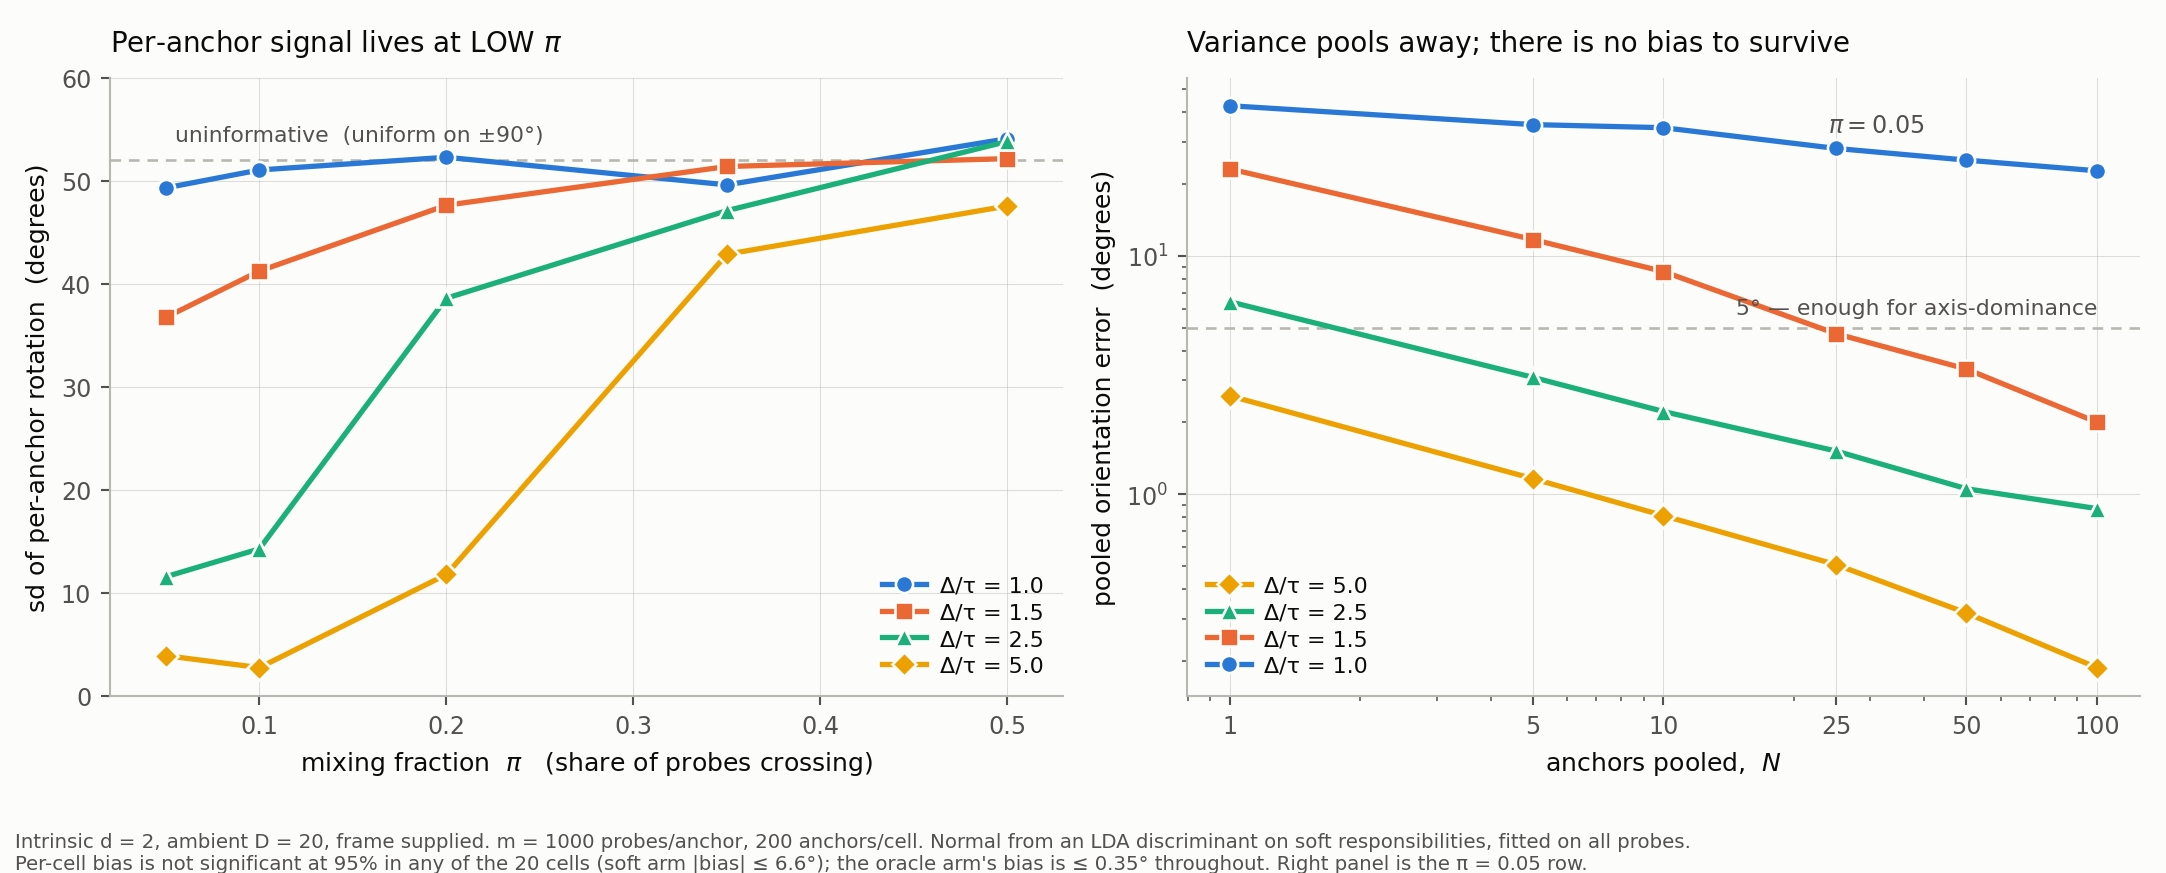
\includegraphics[width=\textwidth]{fig_normal_estimator.png}
\caption{\textbf{Left:} per-anchor information against the mixing fraction. Signal lives at
\emph{low} $\pi$; $52^\circ$ is what uniformly random directions give. \textbf{Right:}
pooled orientation error against the number of anchors, at $\pi = 0.05$.}
\end{figure}

\paragraph{Where the useful anchors are, and it is not where one would guess.} \NEWT\
Per-anchor orientation error is \textbf{monotone increasing in $\pi$}, not U-shaped: at
$\Delta/\tau = 5$ the per-anchor standard deviation runs $3.9^\circ$ at $\pi = 0.05$ to
$47.5^\circ$ at $\pi = 0.50$. Fewer crossers, but they sit much further out along the
normal, and the separation of class-conditional means along $n$ \emph{rises} as $\pi$ falls:

\begin{center}\small
\begin{tabular}{@{}lccccc@{}}
\toprule
$\pi$ & 0.05 & 0.10 & 0.20 & 0.35 & 0.50\\
\midrule
mean separation along $n$ & $2.17\sigma$ & $1.95\sigma$ & $1.75\sigma$ & $1.63\sigma$ & $1.60\sigma$\\
\bottomrule
\end{tabular}
\end{center}

\noindent At $\pi \to 0.5$ there is additionally no majority branch for LTS to commit to, so
the plane lands between branches and corrupts the residuals the mixture sees. The useful
anchors sit at $d \approx 1.3\text{--}1.6\,\sigma$. This agrees with the distance estimator,
which is also most accurate at larger $d/\sigma$, so a single rung serves both.

\paragraph{Weight.} $w_a$ is the LRT statistic, \textbf{not thresholded}. At per-anchor power
near $0.5$, thresholding before pooling discards half the true signal.

\medskip
\noindent Every anchor emits $(n_a, c_a, \dhat_a, \Dhat_a, w_a)$---\textbf{including anchors that
did not fire.}

\section{Stage 5 --- three consistency checks, all free}
\label{sec:stage5}

The $S = 3$ ladder supports three checks on queries already spent. They test different things,
and none is tuned.

\subsection*{(a) How the response scales with radius}

Regress $\log\Dhat$ on $\log r$ across rungs; report the exponent $\alpha$.

\begin{table}[h]
\small\centering
\begin{tabular}{@{}lccc@{}}
\toprule
\textbf{\sffamily Structure} & $\Dhat$ \textbf{\sffamily scaling}
  & \textbf{\sffamily ratio at} $r/2$ & \textbf{\sffamily ratio at} $r/4$\\
\midrule
step (top-1 gate)      & $r^0$ & 1.00 & 1.00\\
kink (top-2 softmax)   & $r^1$ & 0.50 & 0.25\\
curvature (confound)   & $r^2$ & 0.25 & 0.06\\
\bottomrule
\end{tabular}
\end{table}

\noindent Observed: gates $1.01$; resonant curvature $0.04$ at $r/4$ against $r^2$'s predicted
$0.0625$. The log-log regression is preferable to a single-ratio threshold---free, more robust,
and three-way rather than binary.

\subsection*{(b) Whether the geometry is self-consistent \textnormal{\NEWT}}

For a planar boundary at fixed distance, $\dhat_s$ should not depend on the rung. A gate returns
the same $d$ at every scale; a smooth confound's $\pihat_s$ is a mixture fit to something that is
not a crossing, so its implied distance wanders. Measured 13~August:

\begin{table}[h]
\small\centering
\begin{tabular}{@{}lcc@{}}
\toprule
\textbf{\sffamily Model} & \textbf{\sffamily median CV of} $\dhat$ & \textbf{\sffamily fire rate}\\
\midrule
\textbf{gated} & \textbf{0.098} \ (0.074 at $\tau = 0.02$) & 0.678\\
GP null, $\ell = 0.05$, $A = 0.10$ & 0.557 & 0.397\\
GP null, $\ell = 0.05$, $A = 0.20$ & 1.042 & 0.114\\
kink control & 1.241 & 0.023\\
honest & --- & \textbf{0.000}\\
GP null, $\ell = 0.30$ (above ladder top) & --- & \textbf{0.000}\\
\bottomrule
\end{tabular}
\end{table}

\noindent At $\mathrm{CV} < 0.15$: \textbf{56\% of gates retained, 93\% of confounders rejected.}
As a standalone filter that is expensive; its value is as one of three orthogonal checks, and the
operating point should be set after the full pipeline exists---trimming will sharpen $\pihat$ and
will move it.

\begin{figure}[!ht]
\centering
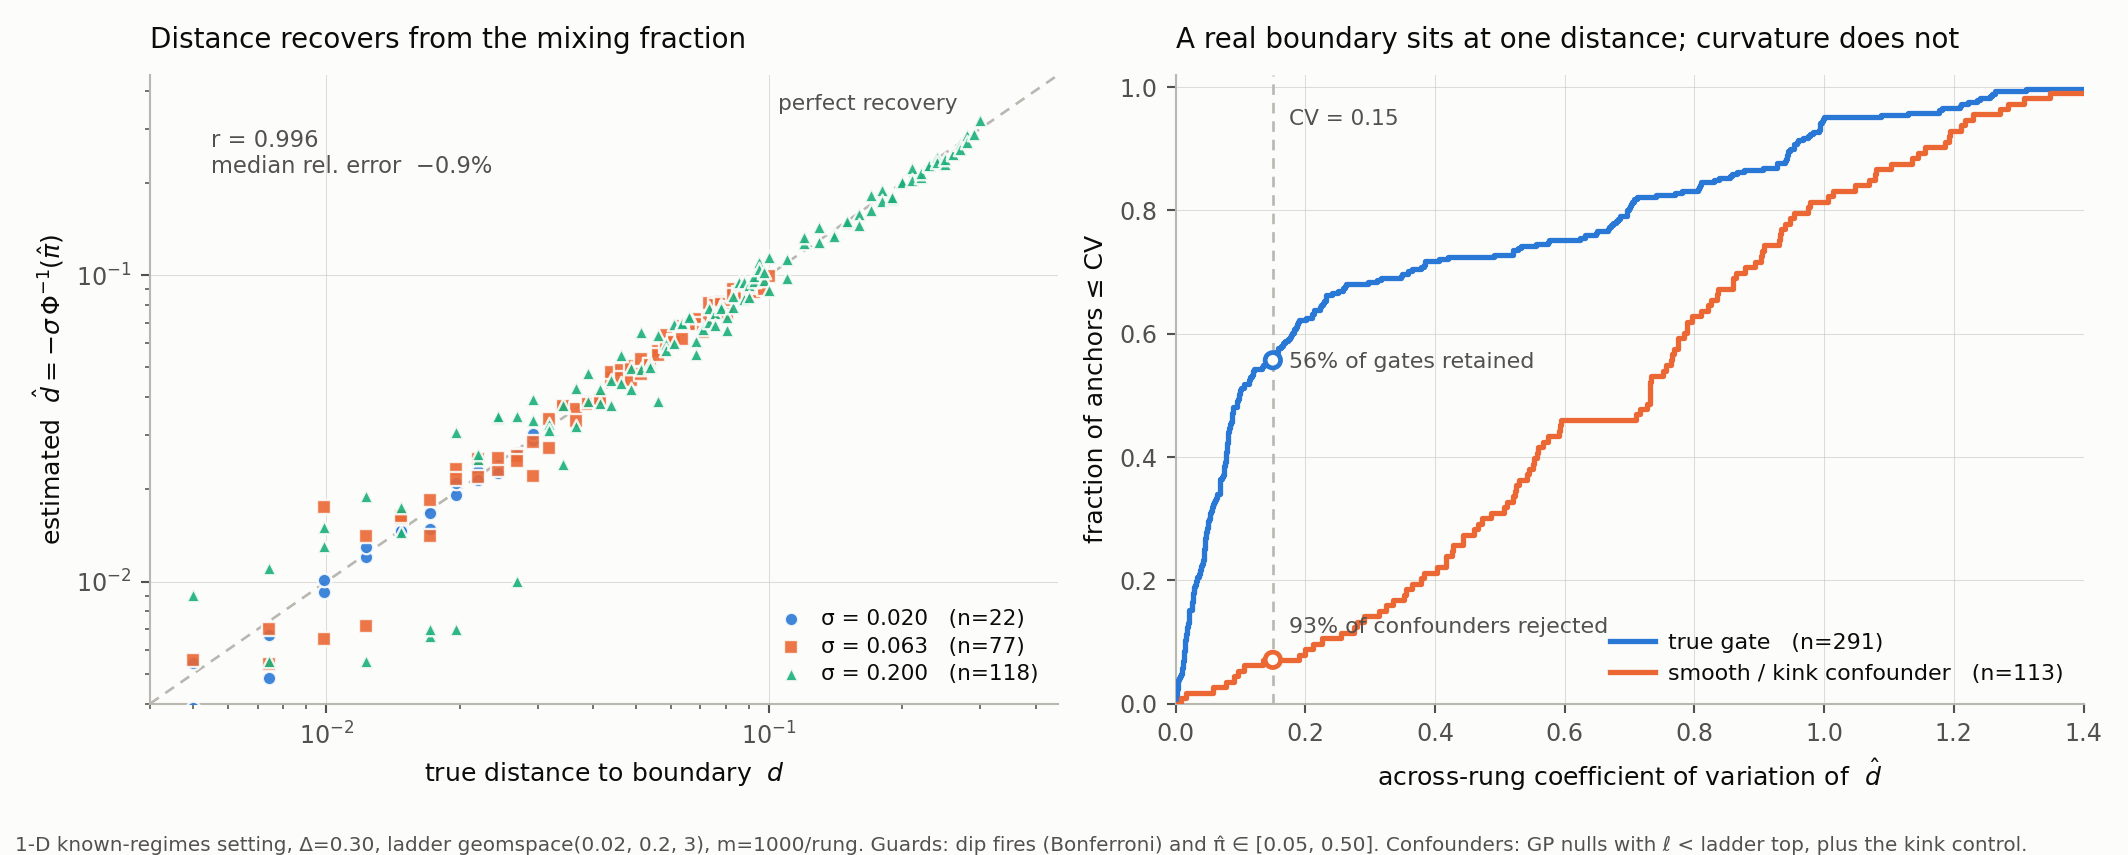
\includegraphics[width=\textwidth]{fig_distance_estimator.png}
\caption{\textbf{Left:} the distance estimator against ground truth, by probe scale. \textbf{Right:}
across-rung constancy of $\dhat$ separates a true gate from smooth and kink confounders.}
\end{figure}

\subsection*{(c) Whether the two routes to the offset agree \textnormal{\NEWT}}

The offset is available twice: from the classifier's own intercept $b/\lVert\nu\rVert$, and from
$-\sigma\Phi^{-1}(\pihat)$ signed by $\nhat$. Both are functionals of the same responsibilities,
so under a correctly specified model they agree by construction---but they \emph{diverge
differently} under misspecification, the way method-of-moments and maximum likelihood do. A large
gap says the boundary is not planar inside the ball, or the mixture is spurious. This is a
specification check, not two independent samples, and should be described as such.

\medskip
\noindent Failing any of the three routes to \texttt{A5\_structure\_unattributed}---structure
present, not attributable to a boundary. A third outcome: not a flag, and not a clean bill.

\section{Stage 6 --- pooling}
\label{sec:stage6}

\SPEC\ A boundary is a shared object: one hyperplane passes through many probe balls. Per-anchor
power of $0.5$ barely matters if evidence for a \emph{common} boundary aggregates over 200
anchors---which means \textbf{per-anchor power is the wrong figure of merit}. The right one is the
number of anchors needed to recover the boundary.

Do not threshold before pooling. All anchors contribute, weighted by $w_a$.

\begin{table}[h]
\small\centering
\begin{tabular}{@{}cp{0.52\textwidth}p{0.30\textwidth}@{}}
\toprule
& \textbf{\sffamily Estimator} & \textbf{\sffamily Uses geometry}\\
\midrule
A & Fisher/Stouffer combination of per-anchor $p$-values & no --- baseline\\
B & threshold on $w_a$, then cluster $(n,c)$ & partly\\
C & $w$-weighted mode-seeking (mean-shift / Hough) over all anchors & fully\\
\bottomrule
\end{tabular}
\end{table}

\noindent Predicted ranking $C > B > A$ at every $\Delta$, with the largest gap at
$\Delta = 1.5$ sd, where half the true detections sit below any per-anchor threshold and $B$
throws them away.

\paragraph{A no-information guard is required.} \NEWT\ Outside the operating region ---
$\Delta/\tau = 1.0$ at any $\pi$, or $\pi \gtrsim 0.35$ --- the per-anchor rotation has
standard deviation $\approx 52^\circ$, which is exactly what uniformly random directions
give. Pooling \emph{axial} estimates that carry no information does not converge to the
truth and does not converge to nothing: the mean direction of $N$ random axes is itself
uniformly random, so the pooled estimate lands on an arbitrary direction with an interval
that tightens around it. \textbf{Pooling can therefore be confidently wrong in a way that
per-anchor abstention never is.} Stage 6 needs an explicit check that the anchor set carries
information before it reports --- the permutation null is the natural instrument, since
uninformative input should be indistinguishable from permuted input.

\paragraph{Null.} Permute the residual-to-point assignment within each anchor and rerun the
pipeline. This randomises normals while preserving marginal residual distributions;
$\ge 500$ permutations.

\paragraph{Metrics.} $N \mapsto$ orientation error, $N \mapsto |\chat - c^\star|$, and $N_{95}$.
The first two are the estimation curves; $N_{95}$ is the detection curve. Under this note's
framing, the first two are the headline.

\paragraph{One warning, stated as a prediction to register rather than a result.} The naive
argument for pooling---real boundaries give consistent normals, artifacts give random ones---
\textbf{fails for the confound that matters}. A resonant surface $0.5\sin(2\pi u_1/\ell)$ has a
preferred direction, so every anchor on it produces a normal aligned with $\pm u_1$. Those pool
\emph{coherently} into a confident false boundary.

The offsets should not agree, though. A gate places every $c_a$ at the same value; a sine places
them at its steep parts, spaced by $\ell$:
\[
  \text{gate} \;\longrightarrow\; \text{a single mode in } c,
  \qquad
  \text{resonant curvature} \;\longrightarrow\; \text{a comb of modes spaced by } \ell .
\]
Register this before running. If it fails, smooth rejection returns to Stage~5 and the per-anchor
decision rules are back on the critical path.

\section{Stage 7 --- stating the rule}
\label{sec:stage7}

\begin{codebox}
\begin{verbatim}
axis-dominance:  is one |n_hat_i| dominant?
                 calibrate against the permutation
                 distribution of max_j |n_hat_j|

if yes:  coordinate i, threshold t_hat = c_hat / n_hat_i,
         CI from the bootstrap
if no:   report the hyperplane (n_hat, c_hat),
         no single-coordinate claim
\end{verbatim}
\end{codebox}

\part{What must still be true}

\section{The obligation the reframe creates}
\label{sec:obligation}

A detector is validated by power and false-positive rate. \textbf{An estimator is validated by
bias, variance, interval coverage, and query complexity}---and three of those four have never been
measured here.

Coverage matters most and has been touched least. The $\pm 0.07$ in the target sentence is doing
enormous work: it is what turns a point estimate into a scientific claim. If the bootstrap
interval on $\that$ does not cover at its nominal rate, that sentence is false in a way a reviewer
will find immediately.

\begin{claimbox}
\noindent \textbf{Calibrated coverage of the interval on $(\nhat, \chat, \that)$ is a first-class
deliverable, not a finishing touch.} Under the detector framing, nothing required it.
\end{claimbox}

\section{The critical path}
\label{sec:path}

\begin{enumerate}
\item \textbf{Validate $\dhat = -\sigma\Phi^{-1}(\pihat)$.} \textcolor{okgreen}{Done 13~August}
(\S\ref{sec:stage4}).
\item \textbf{Validate the separability-derived normal.} \textcolor{okgreen}{Done 13~August}
(\S\ref{sec:stage4}): no detectable bias in any cell, and pooled error below $3^\circ$ at
$N = 100$ down to $\Delta/\tau = 1.5$. Intrinsic $d = 2$ only --- the sweep over
$d \in \{4, 8\}$ is a parameter change in the same harness and remains to be run.
\item \textbf{Experiment P} $\to$ $N \mapsto$ orientation error, $N \mapsto |\chat - c^\star|$,
$N_{95}$. \emph{Revise the distance axis:} the design specified anchor distance
$/\,r_{\text{hi}} \in \{0.2, 0.5, 0.9, 1.5\}$, whose small values place anchors close to the
boundary --- which \S\ref{sec:stage4} shows is exactly where orientation is worst. Sample
the low-$\pi$ region instead.
\item \textbf{Axis-aligned threshold recovery with a \emph{calibrated} interval.}
\end{enumerate}

\paragraph{On deferring Stage 0.} The order above proves geometry recovery first under
\emph{known-valid} local probes---a flat manifold of known dimension, where the frame and radius
can be supplied rather than estimated---and adds automatic geometry selection afterwards. This is
deliberate: the contribution is that $(\nhat,\chat)$ is recoverable at all, and establishing that
under a hand-supplied probe geometry isolates it from any question about how the geometry was
chosen. Stage~0 is then the extension that \emph{removes} the assumption, converting ``given a
valid local probe geometry'' into a condition the method checks for itself and declines when it
fails. Deferred, not dropped: \S\ref{sec:stage0} remains the specification, and the results in
steps 2--4 must state the conditioning explicitly. The one part of Stage~0/1 kept regardless is
the \textbf{density filter}, because it scopes the claim rather than improving it.

\paragraph{Where the error budget lives --- answered.} \emph{The prediction below was made
before step 2 and is retained with its outcome.} Responsibilities are
\emph{estimated}, not true branch labels. The chain runs: mixture misassignment $\to$ classifier
label noise $\to$ bias in $\nhat$. Near weak separation the responsibilities go diffuse
($\gamma \approx 0.5$ almost everywhere) and the discriminant direction destabilises; this may
dominate finite-sample error entirely in the regime that matters. The clean way to isolate it is to
\textbf{fit the classifier twice}---once on estimated responsibilities, once on true labels---and
difference the orientation errors, as a function of $\Delta/\tau$ and $\pi$, not only $N$. If that
gap is large at $\Delta = 1.5$ sd, pooling must weight by \emph{assignment confidence} rather than
by the LRT statistic alone.

\emph{Outcome:} the gap is entirely variance. Bias is not significant in any cell, so
weighting by the LRT statistic is not disqualified, and the binding constraint turns out to
be anchor \emph{placement} ($\pi \le 0.10$) rather than the weighting rule.

\section{Scope: this is a locally single-boundary method}
\label{sec:scope}

\begin{limitbox}
\noindent The procedure identifies \textbf{at most one boundary per probe ball}. Its precondition
is $r_{\text{hi}} < L$, where $L$ is the routing cell scale---and that precondition \textbf{is not
checkable from the covariates alone}, because routing density lives in the response while
covariate geometry is unchanged. \LIMIT
\end{limitbox}

\noindent When it is violated---many experts, small cells, a ball spanning several---the many
small-separation components read as heteroscedastic noise, and \textbf{Stage 0 is blind. No
abstention fires.} This is the only failure mode in the method that returns a confident wrong
answer rather than declining to answer.

Two things follow. It explains why $K = 2$ globally is the right scope rather than an arbitrary
simplification: the local procedure never sees more than one boundary regardless, so global $K$
must be \emph{assembled} from local evidence, never fitted as a large mixture. And it suggests a
response-side detector that does not yet exist---if a ball spans several cells, $\Dhat$ may shrink
with $r$ rather than staying flat, which the existing ladder would see. Worth testing in the
step-2 harness; not claimed. \OPENT

\section{Everything else that limits the claim}
\label{sec:limits}

\begin{itemize}
\item \textbf{Parallel penalty.} An offset aligned with strong within-branch variation is invisible
at every radius, in every dimension, under every projection. Proven, not conjectured. \LIMIT
\item \textbf{Reach is not validity.} The plateau says where assumptions hold, not where the gate
lives. \LIMIT
\item $\bm{\pi \approx 0.5}$\textbf{.} LTS breakdown is structural. The LRT fixes \emph{testing}
($0.32$, graceful); recovery still breaks, since there is no majority branch to trim toward.
\LIMIT
\item \textbf{Detection floor} $\approx 1.5$ sd at $m \sim 10^3$. Moment $z$-scores scale like
$\sqrt{n}$, so halving the detectable separation costs $4\times$ the queries.
\item \textbf{Coverage.} Randomly placed anchors contain a boundary about $r_{\text{hi}}/L$ of the
time---roughly 15--20\%. Fine for detection; a real constraint on constructive recovery.
Boundary-seeking placement does not exist and is a \emph{deployment} problem: in simulation the
boundary is known, so anchors are placed by design. \OPENT
\item \textbf{Validation scope.} One model class, one $D$, one $\tau_y$, and no full-pipeline
bootstrap yet. \OPENT
\end{itemize}

\section{Provenance summary}
\label{sec:provenance}

\begin{table}[h]
\small
\begin{tabular}{@{}p{0.56\textwidth}p{0.38\textwidth}@{}}
\toprule
\textbf{\sffamily Component} & \textbf{\sffamily Status}\\
\midrule
Crossing law; fixed-per-coordinate budget mandatory & \VALID\ to three decimals\\
Trimmed residualisation, dimension-independent power & \VALID\ $0.74$--$0.76$ flat in $D$\\
OLS absorbs ${\sim}64\%$ of the gap & closed form, matches measurement\\
Trimming restores validity on clumpy manifolds & \VALID\ $0.49 \to 0.00$\\
Dispersion cannot discriminate a gate from curvature & \LIMIT\\
Dip floor ${\sim}2$ sd; LRT $0.42$--$0.54$ at $1.5$ sd
  & measured; \textbf{LRT uncalibrated through pipeline}\\
Local $\Dhat$ recovery & \VALID\ $0.291$ vs $0.300$\\
Group-conditional estimand at the anchor & \VALID\ cosine $1.000$\\
\textbf{Distance estimator} $\bm{\dhat = -\sigma\Phi^{-1}(\pihat)}$
  & \VALID\ \textbf{$r = 0.996$, median rel.\ error $-0.9\%$}\\
\textbf{Distance invariance across rungs} & \VALID\ \textbf{CV $0.098$ vs $0.56$--$1.24$}\\
Round-consistency plateau; rank-decade $W$; A1/A1n split & \NEWT, unimplemented\\
Stage 0 entire (GRIDE, plateau, frame) & \SPEC\ --- no implementation exists\\
\textbf{Boundary normal from the separability classifier}
  & \VALID\ \textbf{no bias in 20/20 cells}\\
Pooled orientation error $< 3^\circ$ at $N = 100$, $\Delta/\tau \ge 1.5$ & \VALID\ (at $d = 2$)\\
Discriminant on all probes, not LTS inliers & \NEWT\ $5.8^\circ$ vs $21.9^\circ$\\
Orientation error monotone increasing in $\pi$ & \VALID\ --- prediction of a U-shape falsified\\
No-information guard for pooling & \NEWT\ --- required, not yet designed\\
Intrinsic-dimension scaling of orientation error & \OPENT\ --- $d = 2$ only\\
Offset-agreement check & \NEWT\\
Pooling, permutation null, $N_{95}$ & \SPEC\ --- Experiment P\\
Comb-versus-single-mode discriminator & \NEWT\ --- register before running\\
Axis-dominance and threshold recovery & \NEWT\\
\textbf{Interval coverage on} $\bm{(\nhat,\chat,\that)}$
  & \textbf{never measured} --- \S\ref{sec:obligation}\\
\bottomrule
\end{tabular}
\end{table}

\end{document}
